\documentclass[12pt]{article}
\usepackage{amsmath,amssymb,amsthm,amscd}
\usepackage{tikz}
\usetikzlibrary{intersections,calc,arrows.meta}

\newcommand{\id}{\mathrm{id}}

\begin{document}

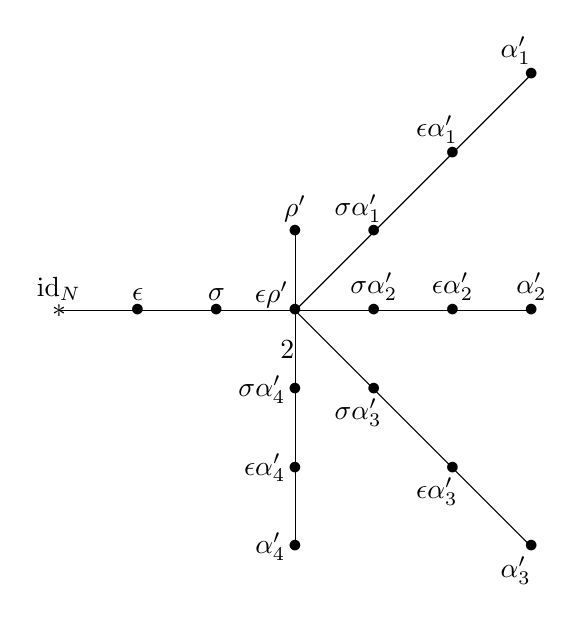
\begin{tikzpicture}
\draw (-3,0)--(-2,0)--(-1,0)--(0,0)--(1,0)--(2,0)--(3,0);
\draw (0,0)--(1,1)--(2,2)--(3,3);
\draw (0,0)--(1,-1)--(2,-2)--(3,-3);
\draw (0,1)--(0,0)--(0,-1)--(0,-2)--(0,-3);
\draw(-3,0)node{$*$};
\draw(-2,0)node{$\bullet$};
\draw(-1,0)node{$\bullet$};
\draw(0,0)node{$\bullet$};
\draw(1,0)node{$\bullet$};
\draw(2,0)node{$\bullet$};
\draw(3,0)node{$\bullet$};
\draw(1,1)node{$\bullet$};
\draw(2,2)node{$\bullet$};
\draw(3,3)node{$\bullet$};
\draw(1,-1)node{$\bullet$};
\draw(2,-2)node{$\bullet$};
\draw(3,-3)node{$\bullet$};
\draw(0,1)node{$\bullet$};
\draw(0,-1)node{$\bullet$};
\draw(0,-2)node{$\bullet$};
\draw(0,-3)node{$\bullet$};
\draw(-0.1,-0.5)node{2};
\draw(-3,0)node[above]{$\id_N$};
\draw(-2,0)node[above]{$\epsilon$};
\draw(-1,0)node[above]{$\sigma$};
\draw(-0.3,0.2)node{$\epsilon\rho'$};
\draw(0,1)node[above]{$\rho'$};
\draw(0.8,1.3)node{$\sigma\alpha_1'$};
\draw(1.8,2.3)node{$\epsilon\alpha_1'$};
\draw(2.8,3.3)node{$\alpha_1'$};
\draw(1,0)node[above]{$\sigma\alpha_2'$};
\draw(2,0)node[above]{$\epsilon\alpha_2'$};
\draw(3,0)node[above]{$\alpha_2'$};
\draw(0.8,-1.3)node{$\sigma\alpha_3'$};
\draw(1.8,-2.3)node{$\epsilon\alpha_3'$};
\draw(2.8,-3.3)node{$\alpha_3'$};
\draw(0,-1)node[left]{$\sigma\alpha_4'$};
\draw(0,-2)node[left]{$\epsilon\alpha_4'$};
\draw(0,-3)node[left]{$\alpha_4'$};
\end{tikzpicture}

\end{document}